\documentclass[dvipdfmx]{beamer}


%%%%% VIEW %%%%%
\usetheme{Montpellier}
\usecolortheme{crane}
\usefonttheme{professionalfonts} % Math Font
\setbeamertemplate{footline}[frame number] % only frame number in footer
\setbeamertemplate{navigation symbols}{} % remove navigation symbol
\renewcommand{\familydefault}{\sfdefault}% font chenge to Sans-serif in English
\usepackage[deluxe,expert]{otf}
\renewcommand{\kanjifamilydefault}{mg}% font chenge to hiragino in Japanese

\setbeamertemplate{caption}[numbered]
%%%%% Fiture, Table Title Rename %%%%E%
\renewcommand{\figurename}{図}
\renewcommand{\tablename}{表}

\usepackage{bm} % Bold charactor package for math
\usepackage{color}

\usepackage[footnotesize, bf]{caption}
\newcommand{\argmin}{\mathop{\rm arg~min}\limits}

%%%% Definition %%%%%
\usepackage{amsmath,amssymb}
\usepackage{amsthm}
\theoremstyle{definition}

\title{PRML Seminar \#1}
\subtitle{ 1.1-1.6.1 \quad \#PRML学ぼう}
\author{Shunya Ueta}
\institute{Graduate School of SIE, Univ. of Tsukuba \\ Department of Computer Science}
\date{\today} % Print Build time

%%%%% Start Slide part %%%%%

\begin{document}

\begin{frame}
  \titlepage % Generated Title Page by preamble params
\end{frame}

\begin{frame}
  \tableofcontents % Generated tabele of contents by section tag
\end{frame}

\section{Introduction}

\begin{frame}
  \frametitle{自己紹介}
    \begin{itemize}
      \item 名前:上田隼也(@hurutoriya)
      \item 筑波大学大学院1年 Go to Doctor course :)
      \item 情報数理研究室所属
      \item 研究分野 : 画像認識・機械学習
    \end{itemize}
\end{frame}

\subsection{この勉強会について}

\begin{frame}
  \frametitle{この勉強会について}
  \begin{itemize}
    \item パターン認識と機械学習についての輪講です \\
    機械学習とパターン認識の基礎を理解、実用レベルで使いこなす事を目的にセミナーを開催していきます
    \item 2015年を目処に一周予定
    \item 受講者には基礎的な微積分・線形代数・確率統計の知識を前提としています
    \item 資料中のサンプルコードはPythonを採用しています。
    \item 勉強会に関する情報については Hashtag: \textcolor{blue}{\#PRML学ぼう} を使って発信していきます
  \end{itemize}
\end{frame}

\subsection{PRML輪講 \#2 内容}
\begin{frame}
  \frametitle{今回の担当}
  \begin{figure}[htb]
    \centering
    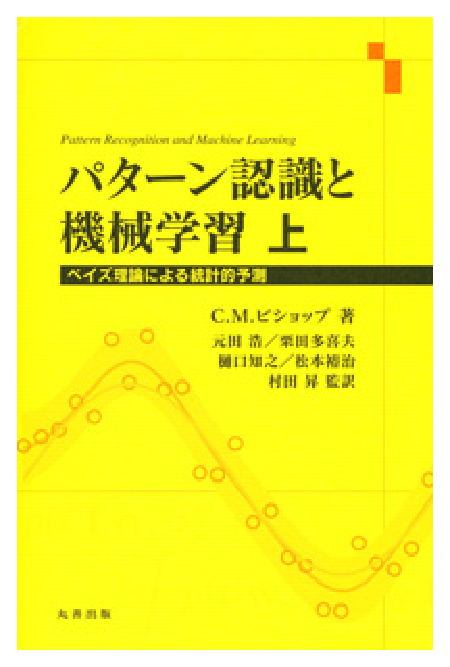
\includegraphics[width=2.5cm,clip]{res/prml.eps}
  \end{figure}
  1.1-2.3.4. (長すぎてダレるかもしれません。でも頑張ります)
\end{frame}

\section{第$1$章 \enspace 序論}

\begin{frame}
  \frametitle{機械学習とは?}
  パターン認識(Pattern Recognition): \\ 計算機アルゴリズムを通じて、データの中の規則を\textcolor{blue}{自動的}に見つけ出す。更にその規則性を用いてデータを異なるカテゴリに分類する。
  \\
  例) 手書き数字の認識
   
  入力として$28 \times 28$ の大きさの手書き数字の画像がある。入力データは$784$次元の実数値ベクトル$x$で表現できる。ベクトル$\bm{x}$を入力として受け取り、それが$0 \ldots 9 $のどの数字を表しているかを出力する機械を作る。
  \begin{figure}[htb]
    \centering
    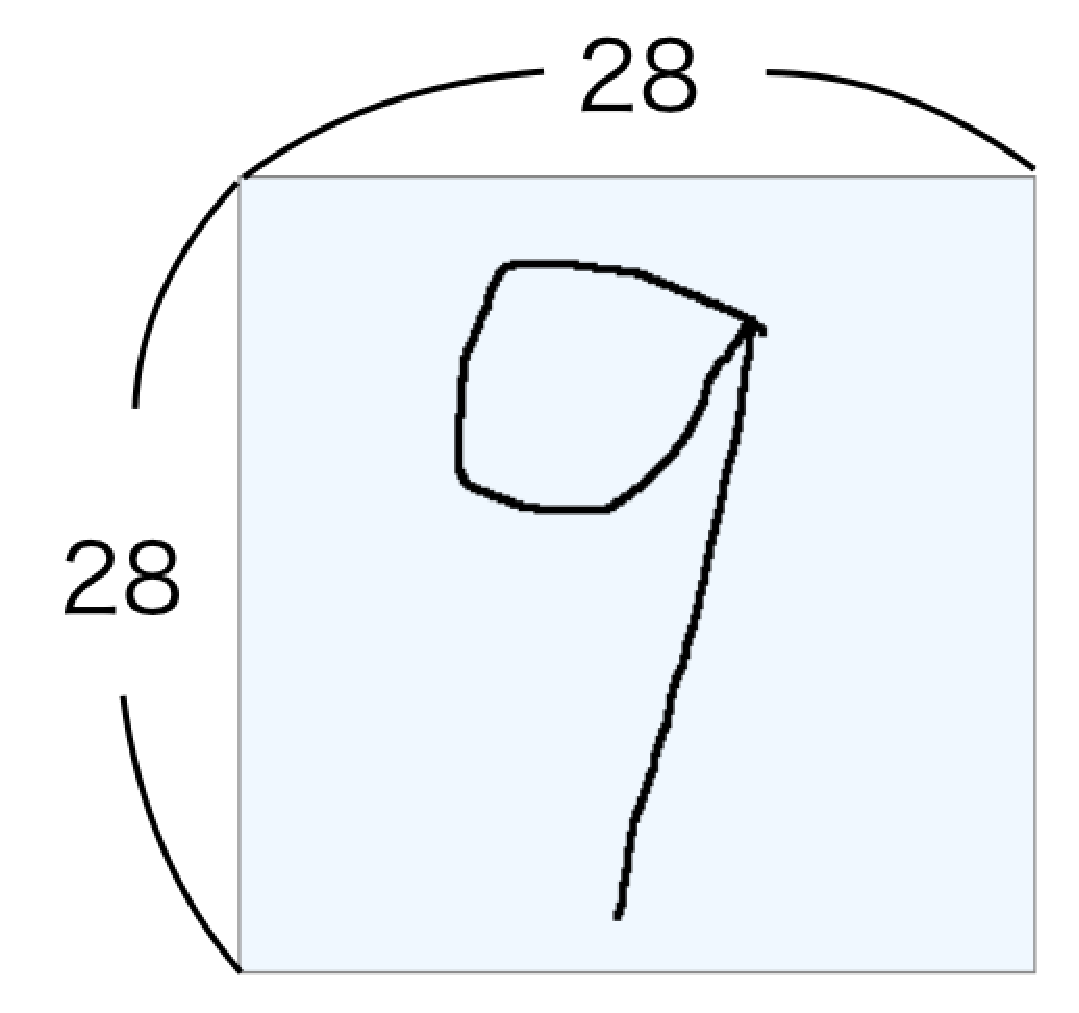
\includegraphics[width=1.5cm,clip]{res/handwritten.eps}
    \caption{手書き数字の画像例}
  \end{figure}
\end{frame}

\begin{frame}
  \frametitle{実現方法(1)}
  人力によるルールの作成 $\to$
  ルール数の発散(\textcolor{red}{実現不可})
  \\
  
  \begin{block}{機械学習的アプローチ}
    \begin{itemize}
      \item 訓練集合(training set):\\$N$個の手書き文字の大きな集合を用意する
      $\{x_1, \ldots , x_N \}$
      \item  目標ベクトル(target vector): $\bm{t}$ \\
      一つ一つの数字に対応するカテゴリを表すベクトル
    \end{itemize}
  \end{block}
  最終的に得られるのは$y(x)$である。\\
  この関数に数字の画像$\bm{x}$を入力すると、目標ベクトルと画像データに符号化可能なデータが合成されたベクトル$\bm{y}$(目標ベクトル)がラベリングされた画像が返ってくる。
\end{frame}

\begin{frame}
  \frametitle{実現方法(2)}
    \begin{itemize}
      \item 訓練(training), 学習(leaning) 段階 : \\ training setのみでモデル化されている状態
      \item テスト集合(test set) : \\ 訓練集合以外のデータ(未知のデータ)
      \item 汎化(generalization) : \\ 訓練集合以外のデータ(未知のデータ)に対して適応可能にさせること
    \end{itemize}
     実問題として入力データは大きな多様性を持つ。$\to$ \\ 汎化が中心的な課題となる。
\end{frame}

\begin{frame}
  \frametitle{例)Ajaxを使った手書き文字認識}
  \begin{figure}[htb]
    \centering
    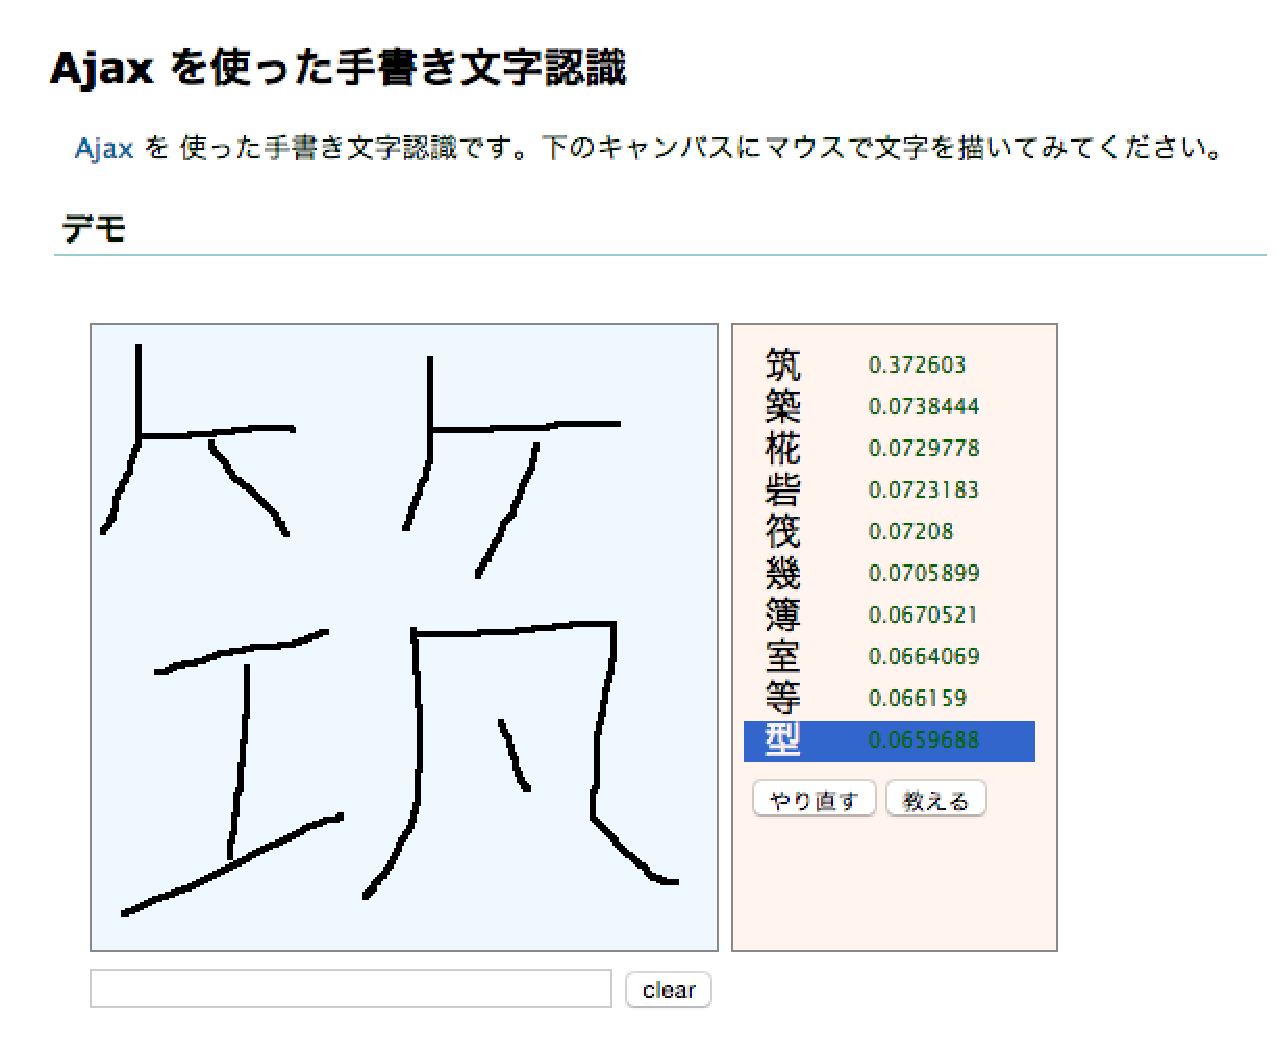
\includegraphics[width=6.0cm,clip]{res/ajax.eps}
    \caption{Ajaxを使った手書き文字認識}
  \end{figure}
  参考: \textcolor{blue}{http://chasen.org/~taku/software/ajax/hwr/}
\end{frame}

\begin{frame}
  \frametitle{前処理(Preprocessing)}
  実世界では、入力変数は\textcolor{blue}{前処理(Preprocessing)}により問題を解きやすくしておく。
  \begin{block}{例)手書き数字}
    \begin{itemize}
      \item 数字画像に変形(アフィン変換)、拡大・縮小を行い \\ 同一の大きさに変換 $\to$ 入力データの多様性の減少
    \end{itemize}
  \end{block}
  前処理の段階は特徴抽出(feature extraction)と呼ばれる。
  
  多様性減少の目的以外にも、計算の高速化のためにも用いられる事が多い。
\end{frame}

\begin{frame}
  \frametitle{機械学習の分類}
  \begin{enumerate}
    \item 教師あり学習(supervised learning) : 訓練データがラベリングされている状態での問題
      \begin{itemize}
        \item クラス分類(classification)問題 : 各入力ベクトルを有限個の離散カテゴリに分類する問題
        \item 回帰(regression) : 求める出力が一つないしはそれ以上の連続変数であるような問題
      \end{itemize}
    \item 教師なし学習(unsupervised learning) : 訓練データがラベリングされている状態での問題
      \begin{itemize}
        \item クラスタリング(clustering) : 類似した事例のグループを見つける
        \item 密度推定(density estimation) : 入力空間におけるデータの分布を見つける
      \end{itemize}
    \item 半教師あり学習(semis-upervised learning) : 訓練データがラベリングされているものと非ラベリング状態の物が混在している状態での問題
  \end{enumerate}
\end{frame}

\begin{frame}
  \frametitle{強化学習(reinforcement learning)(1)}
  教科学習(reinforcement learning) : ある与えられた条件下で、報酬を最大化するような適当な行動を見つける問題。
  \\
  状態と行動の系列から環境との相互作用を通じて学習を行う(行動基準は直近の報酬だけではなく、過去の行動も参考にされる)。
  \\
  教師あり学習との違い : 最適な答えは与えられずに試行錯誤を通じて学習アルゴリズム自らが最適解を発見する

  \begin{block}{バックギャモンに対する強化学習の適用(Tesauro 1994)}
    ニューラルネットワーク(第5章)により、自分自身のコピーと何百万ものゲームをこなす必要がある。\\
    選択肢は無数に存在するが、勝利という形でしか報酬を与えることができない。そのため、勝利に関係する手に対しては正確に報酬を割り当てる必要がある(\textcolor{red}{信頼度割り当て問題})。
  \end{block}
\end{frame}

\begin{frame}
  \frametitle{強化学習(reinforcement learning)(2)}
  下記の2つを行い強化学習を行う(トレードオフの関係)。
  \begin{itemize}
    \item 探査(exploration) : 新規の手がどれほど有効なのかを探す
    \item 利用(exploitation) : 高い報酬が得られることがわかっている行動を取る
  \end{itemize}
\end{frame}

\begin{frame}
  \frametitle{第1章で導入する3つの重要な道具}
  \begin{enumerate}
    \item 確率論
    \item 決定理論
    \item 情報理論
  \end{enumerate}
\end{frame}

\subsection{1.1 多項式曲線フィッティング}
\begin{frame}
  \frametitle{1.1 \ 多項式曲線フィッティング}
  訓練データ \\
  入力 : $N$個の観測値$x$を並べた $\bm{x} = (x_1, \dots, x_N)^T$ \\
  出力 : それぞれに対応する観測値 $\bm{t} = (t_1, \dots, t_N)^T$ \\
 
  未知の入力変数$x$に対して目標変数を予測したい$t$ (汎化)\\
  
  目標とするモデルは$\sin{2 \pi x}$、訓練データはノイズを乗せて$N=10$で与えられる。
  \begin{figure}[htb]
    \centering
    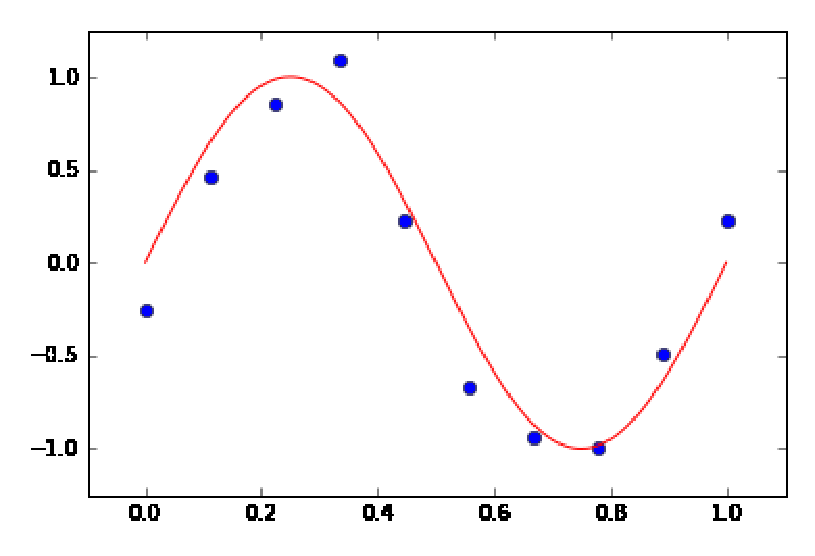
\includegraphics[width=4.0cm,clip]{res/fitting.eps}
    \caption{ex)N=10で訓練データが与えられている}
  \end{figure}
  
\end{frame}

\begin{frame}
  \frametitle{1.1 \ 多項式曲線フィッティング}
  \begin{gather*}
    y(x,\bm{w}) = w_0 x^0 + w_1 x^1 + \dots + w_M x^{M} = \sum_{j=0}^{M} w_j x^j
  \end{gather*}
  $M$:多項式の次数(order) \\
  $\omega$:多項式の係数、まとめて$\bm{\omega}$で表す \\
  \begin{gather*}
    E(\bm{w}) = \frac{1}{2} \sum_{n=1}^{N} \{ y(x_n,\bm{w})- t_n \}^2
  \end{gather*}
  訓練データに多項式をあてはめることで、係数の値を求めたい $\to$ 誤差関数(Error Function)の最小化を目指す。
\end{frame}

\begin{frame}
  \frametitle{Fitting Order Case:M=0,1}
\end{frame}

\begin{frame}
  \frametitle{Fitting Order Case:M=3,9}
\end{frame}

\begin{frame}
  \frametitle{過学習と平均二乗平方根誤差}
  9次でフィッティングした場合、\textcolor{red}{過学習}(over-fitting)
  \\
  \textcolor{blue}{機械学習の目標}:未知のデータに対して精度の高い予測(汎化)
  \begin{gather*}
    E_{RMS} = \sqrt{2E(\bm{w})/N}
  \end{gather*}
  平均二乗平方根誤差(root-mean-square error,RMS error)
  \\
  \begin{itemize}
    \item Nで割ることでサンプル数のギャップを消す
    \item 平方根を取ることで、元の尺度に戻す
  \end{itemize}
\end{frame}
\begin{frame}
  \frametitle{データセットのサイズに応じた過学習の様子}
\end{frame}
\begin{frame}
  \frametitle{誤差関数の正則化(regularization)過学習を制御}
  \begin{gather*}
    E(\bm{w}) = \frac{1}{2} \sum_{n=1}^{N} \{ y(x_n,\bm{\omega})- t_n \}^2 + \frac{\lambda}{2}||\bm{w} ||^2
  \end{gather*}
  2次の正則化の場合、リッジ回帰(ridge regression)
\end{frame}

\begin{frame}
  \frametitle{}
  検証用集合(Validation set):$\bm{w}$を決定するためにデータセット ホールド・アウト集合(hold-out set)とも呼ばれる。
  
  \textcolor{red}{欠点}: 貴重なデータを無駄にする
\end{frame}

\subsection{1.2 確率論}

\begin{frame}
  \frametitle{確率論}
  データにはノイズが必ず付随し、データセットのサイズも有限である。\textcolor{red}{不確実性}が重要な概念となる。
  
  \begin{block}{確率論の概念を簡単に説明}
    \begin{figure}[htb]
      \centering
      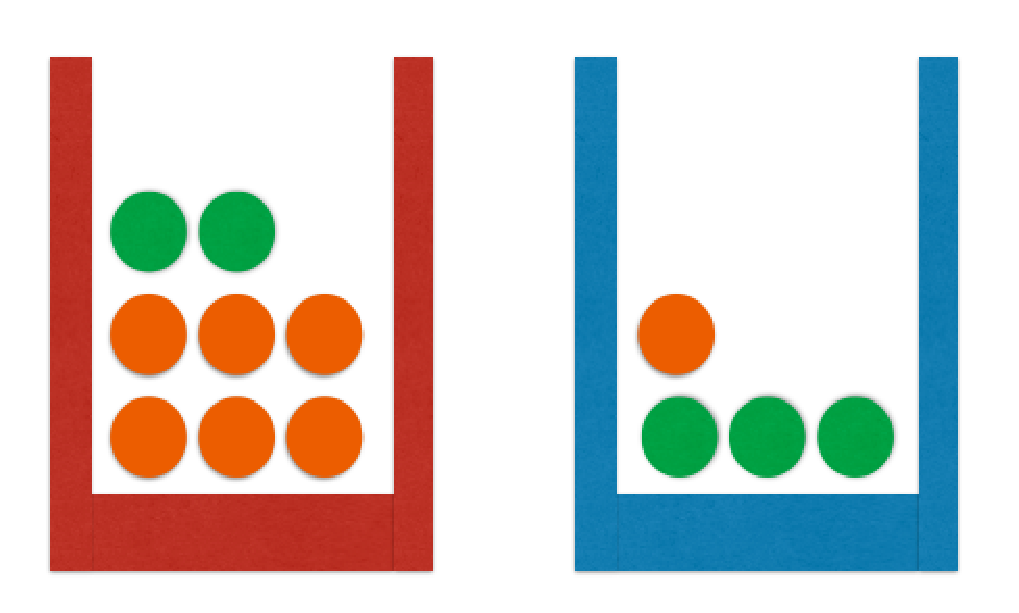
\includegraphics[width=4.0cm,clip]{res/probability.eps}
      \caption{赤と青、2つの箱がある。赤の箱にはりんごが2個、オレンジが6個、青の箱にはりんごが3個、オレンジが一個入っている。赤の箱を40\%,青の箱を60\%で選び、果物は同じ確からしさで選ぶ。}
    \end{figure}
  \end{block}
\end{frame}

\begin{frame}
  \frametitle{確率の基本的法則}
  \begin{description}
    \item[確率の加法定理(Sum rule)]
      \begin{gather*}
        p(X)=\sum_{Y} p(X,Y)
      \end{gather*}
    \item[確率の乗法定理(Prduct rule)]
      \begin{gather*}
        p(X,Y)=p(Y|X)p(X)
      \end{gather*}
    \item[ベイズの定理(Bay's theorem)]
      \begin{gather*}
        p(Y|X) = \frac{p(X|Y)p(Y)}{p(X)}
      \end{gather*}
  \end{description}
\end{frame}
\begin{frame}
  \frametitle{ベイズの定理の直感的な説明}
  \begin{figure}[htb]
    \centering
    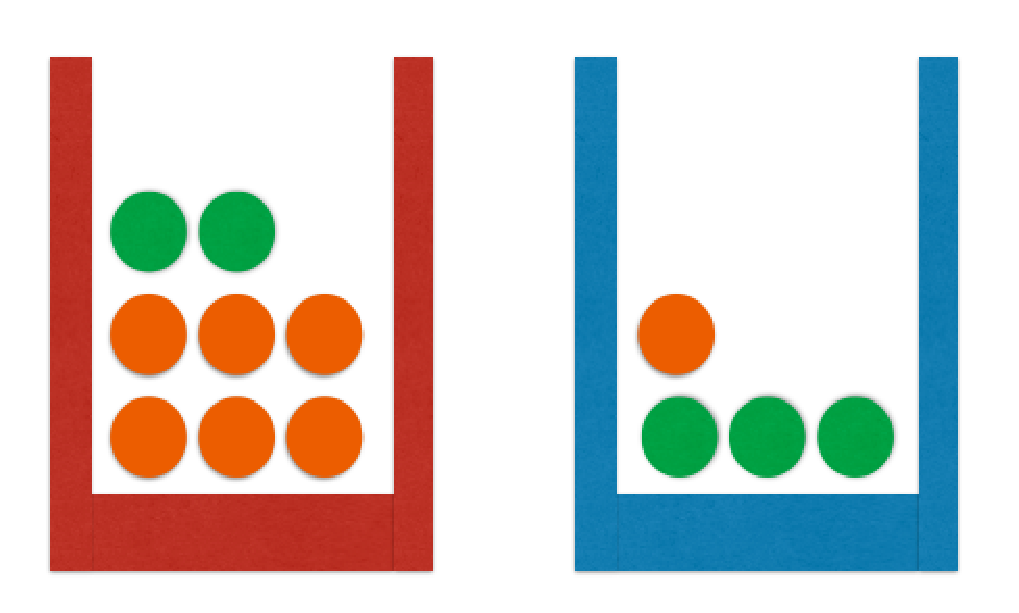
\includegraphics[width=4.0cm,clip]{res/probability.eps}
  \end{figure}
  どの箱を選びましたか?
  \begin{description}
    \item[事前確率(prior probability)] \hfill \\
      事前に得られる確率値 $p(Box)$
    \item[事後確率(posterior probability)] \hfill \\
      果物を選んだ後確定する確率 $p(Box|Fruit)$
  \end{description}
  一旦果物がオレンジだとわかれば、赤い箱はオレンジの数が多い$\to$赤い箱である確率が高くなる。
\end{frame}

\begin{frame}
  \frametitle{1.2.1 連続変数への拡張}
  \begin{description}
    \item[確率密度(probability density) 対象:連続値(continuous value)] \hfill \\
      連続値である変数$x$が区間$(x,x + \delta x)$に入る確率が$\delta x \to 0$で与えられた時の$x$上の$p(x)$
      \\
      \begin{enumerate}
        \item $p(x) \geq 0$
        \item $\int_{-\infty}^{\infty} p(x) dx = 1$
      \end{enumerate}
    \item[確率質量(probability mass) 対象:離散集合(discrete set)] \hfill \\
      離散変数である$x$がある$x$になる確率$p(x)$
    \end{description}
\end{frame}

\begin{frame}
  \frametitle{1.2.2 期待値と分散について}
  \begin{description}
    \item[期待値(expectation)] \hfill \\
      ある関数$f(x)$の確率分布$p(x)$下での平均値
    \begin{description}
      \item[離散分布] $\mathbb{E}[f] = \sum_{x} p(x)f(x)$
      \item[連続変数] $\mathbb{E}[f] = \int p(x)f(x)dx$
    \end{description}
    \item[分散(variance)]
    \begin{align*}
      \rm{var}[f] &= \mathbb{E}[(f(x)-\mathbb{E}[f(x)])^2] \\
                  &= \mathbb{E}[f(x)^2 -2f(x)\mathbb(E)[f(x)]  + \mathbb{E}[f(x)]^2] \\
                  &= \mathbb{E}[f(x)^2 -2f(x)\mathbb(E)[f(x)]  + \mathbb{E}[f(x)]^2] \\
                  &= \mathbb{E}[f(x)^2] -2\mathbb{E}[f(x)]\mathbb(E)[f(x)]  + \mathbb{E}[f(x)]^2 \\
                  &= \mathbb{E}[f(x)^2] -\mathbb{E}[f(x)]^2 \quad \textcolor{blue}{\rm{seminar1.5}}
    \end{align*}
  \end{description}
\end{frame}

\begin{frame}
  \frametitle{共分散(covariance)}
    \begin{align*}
      \rm{cov}[x,y] &= \mathbb{E}_{x,y}[(x-\mathbb{E}[x])(y-\mathbb{E}[y])] \\
                    &= \mathbb{E}_{x,y}[xy + \mathbb{E}[x]\mathbb{E}[y] -x\mathbb{E}[y] -y\mathbb{E}[x]] \\
                    &= \mathbb{E}_{x,y}[xy] +\mathbb{E}_{x,y}[\mathbb{E}[x]\mathbb{E}[y]] -\mathbb{E}_{x,y}[x\mathbb{E}[y]] -\mathbb{E}_{x,y}[y\mathbb{E}[x]] \\
                    &= \mathbb{E}_{x,y}[xy] +\mathbb{E}[x]\mathbb{E}[y] -\mathbb{E}[x]\mathbb{E}[y]] -\mathbb{E}[y]\mathbb{E}[x] \\
                    &= \mathbb{E}_{x,y}[xy] -\mathbb{E}[x]\mathbb{E}[y] \\
                    &= \mathbb{E}_{x,y}[xy] -\mathbb{E}[x]\mathbb{E}[y] (x,y \rm{:independ})\\
                    &= \mathbb{E}[x]\mathbb{E}[y] -\mathbb{E}[x]\mathbb{E}[y] (x,y \rm{:independ})\\
                    &= 0 \quad \textcolor{blue}{\rm{seminar1.6}}
    \end{align*}
\end{frame}

\begin{frame}
  \frametitle{1.2.3 Frequentist VS Bayesian}
  \begin{description}
    \item[Frequentist] \hfill \\
      確率をランダムな繰り返し的試行の頻度とみなす
    \item[Bayesian] \hfill \\
      不確実性の度合いを確率とする
      
      例)\textcolor{red}{この世界に何度も繰り返し行うことができる事象がどれだけあるか考えてみて欲しい。}
      
      南極の氷が喪失するなど不確かな事象が起きたとしよう。年間どの程度溶けているかの情報を得ることで、その情報を適応することで南極の氷が喪失する不確かさを予測する。
  \end{description}
\end{frame}

\begin{frame}
  \frametitle{1.2.3 Likelifood function  working on Frequentist, Bayesian}
  \begin{description}
    \item[尤度関数(likelihood function)] \hfill \\
      $p(Data|param)$ \quad データに対する評価。パラメータの関数とみなせる。
    \item[Frequentist] \hfill \\
      パラメータは固定されているものと考えられている。データの分布を考慮して、パラメータは決定される。
    \item[Bayesian] \hfill \\
      データは唯一に定まり、パラメータに関する不確実性はwの確率分布として表現される。
  \end{description}
\end{frame}

\begin{frame}
  \frametitle{Bayesianの利点}
  事前知識を自然に導入できること

  \begin{block}{例) Frequentistにおける観測に偏りが発生した場合の確率}
    公平に表・裏がでるコインを3回投げて毎回表がでた。古典的な最尤推定では、表が出る確率は1になってしまう。
  \end{block}
  \begin{description}
    \item[尤度] \hfill \\
      尤度は確率と数値的に同じである。
      \\
      例)サイコロを振って1が三回連続同じ物が出る同時確率と尤度は同値である。
      
      違いは、\textcolor{blue}{確率}は「事象の確率」であり、\textcolor{blue}{尤度}は「観測データ下での仮説の尤度」である。

      (likelihood for a hypothesis given a set of observations)
  \end{description}
\end{frame}

\begin{frame}
  \frametitle{1.2.4 Gaussian distribution}
  \begin{gather*}
    N(x|\mu, \sigma^2) = \frac{1}{\sqrt{2\pi \sigma^2}}\exp\{-\frac{1}{2\sigma^2}(x-\mu)^2 \}
  \end{gather*}
  params: $\mu,\sigma^2$
  \begin{figure}[htb]
    \centering
    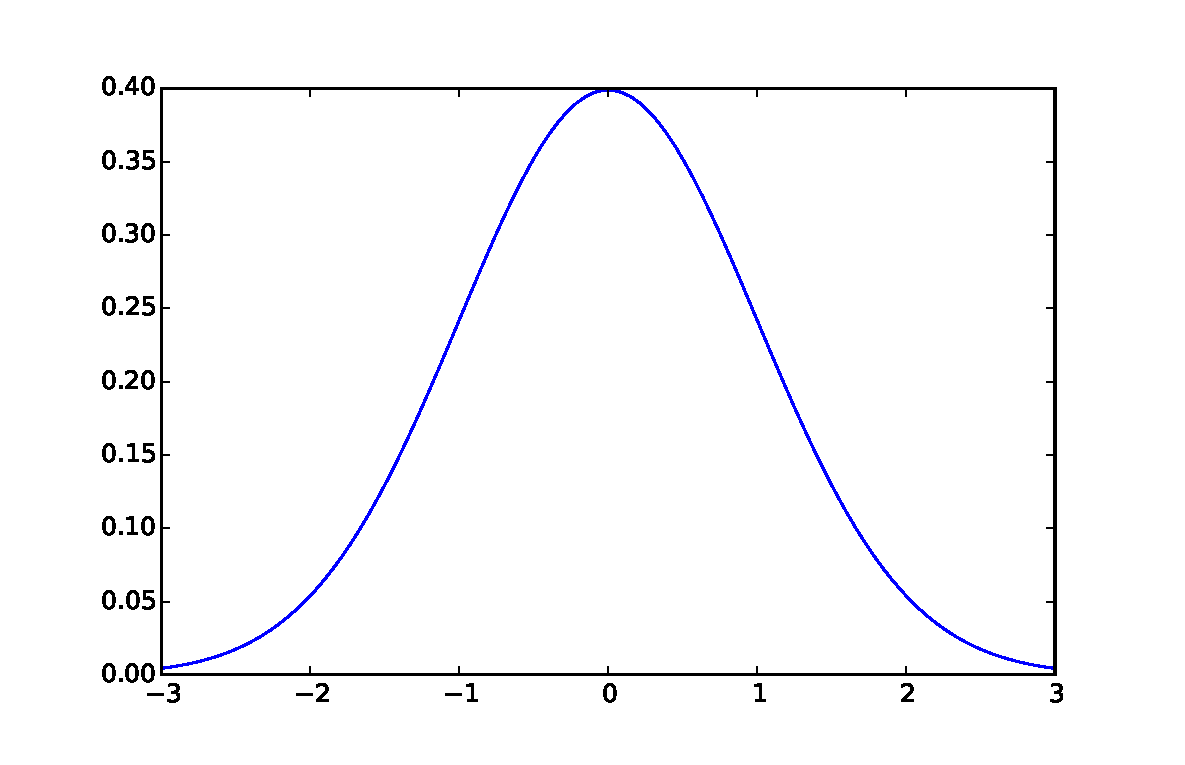
\includegraphics[width=6.5cm,clip]{res/gasussiandist.eps}
    \caption{$\mu =0,\sigma=1$}
  \end{figure}
\end{frame}

\begin{frame}
  \frametitle{1.2.5 Re:Fitting curve}
  Bayesianにおける曲線フィッティング
  \begin{gather*}
    p(t|x,\bm{w},\beta)=N(t|y(x,\bm{w}),\beta^{-1})
  \end{gather*}
  分布の逆分散に相当するパラメータ $\beta$を定義。
  
  訓練データ${\bm{x},\bm{t}}$を使って、未知のパラメータ$\bm{w},\beta$を求めるのに最尤推定を用いる。
  \begin{gather*}
    p(\bm{t}|\bm{x},\bm{w},\beta)=\prod_{n=1}^{N} N(t_n | y(x_n,\bm{w}),\beta^{-1})
  \end{gather*}
\end{frame}

\begin{frame}
  \frametitle{Maximum likelifood function}
  尤度関数を最大化するさいには、対数を用いる。利点として
  \begin{enumerate}
    \item 乗算が加算に変化
    \item 確率は少数で表現されるので、乗算を行うとアンダーフローが頻発
  \end{enumerate}
  \begin{gather*}
    p(\bm{t}|\bm{x},\bm{w},\beta)=\prod_{n=1}^{N} N(t_n | y(x_n,\bm{w}),\beta^{-1})
  \end{gather*}
  \begin{gather*}
    \ln{p(\bm{t}|\bm{x},\bm{w},\beta)} = -\frac{\beta}{2}\sum_{n=1}^{N} \{ y(x_n,\bm{w}) - t_n \}^2 + \frac{N}{2},\ln{\beta} -\frac{N}{2}ln{2\pi}
  \end{gather*}
\end{frame}

\begin{frame}
  \frametitle{予測分布(predictive distribution)}
  パラメータベクトル$\bm{w}_{ML}$をまず決定し、$\beta_{ML}$を推定する。
  \begin{gather*}
    \frac{1}{\beta_{ML}}=\frac{1}{n} \sum_{n=1}^{N} \{ y(x_n,\bm{w}_{ML})- t_n \}^2
  \end{gather*}
  $\beta_{ML}$が決定されたことにより予測分布という形で$t$の確率分布を考えることができる。
  \begin{gather*}
    p(\bm{t}|\bm{x},\bm{w},\beta)=\prod_{n=1}^{N} N(t_n | y(x_n,\bm{w}),\beta^{-1})
  \end{gather*}
\end{frame}

\subsection{1.4次元の呪い}
\begin{frame}
  \frametitle{実世界問題への応用}
  曲線フィッティングでは、入力パラメータは一つ。現実問題では入力パラメータは複数個存在するのが当たり前である。
  
  自分たちは3次元の存在。4次元以上の空間に関しては\textcolor{blue}{幾何的直感}は働きづらい。
  \begin{figure}[htb]
    \centering
    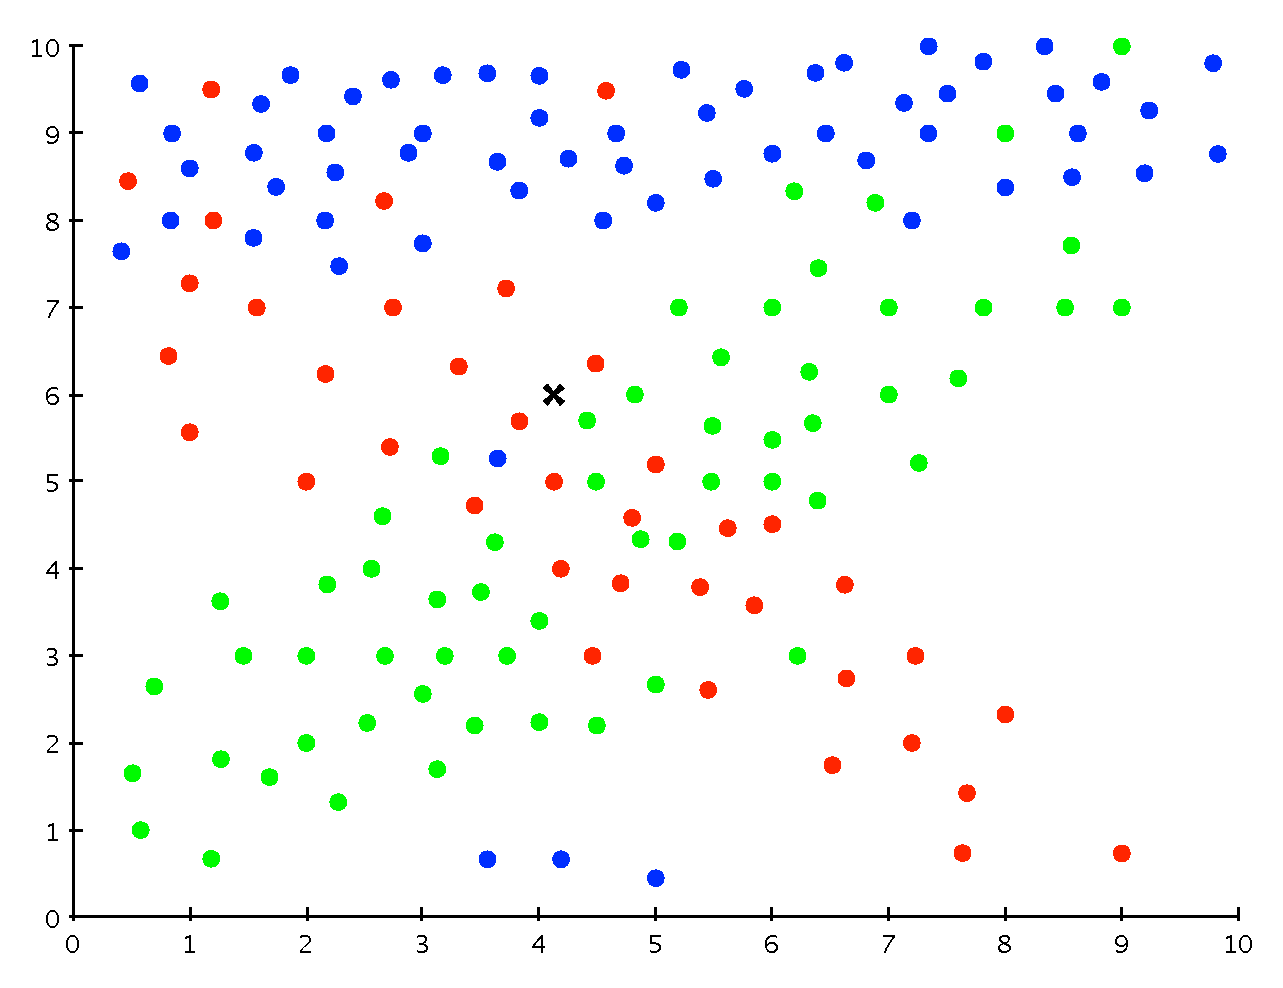
\includegraphics[width=4.5cm,clip]{res/curse_dim.eps}
    \caption{3クラス存在するデータセットの散布図、わかりやすいように2次元の部分空間へ}
  \end{figure}
\end{frame}

\begin{frame}
  \frametitle{割り当て方法の提案}
  \begin{figure}[htb]
    \centering
    \includegraphics[width=4.5cm,clip]{res/curse_dim_grid.eps}
    \caption{同グリッド内で最も多いクラスを割り当てる}
  \end{figure}
  高次元に有効な2つの性質
  \begin{enumerate}
    \item 実データでも有効なデータは低次元に集中している
    \item データは滑らかな事が多い(局所的に)ので、内挿により対応する \hfill \\
      学習モデルを適用する必要はなく、内挿で事足りる
  \end{enumerate}
\end{frame}
\subsection{1.5 決定理論}
\begin{frame}
  \frametitle{About decision theory}
  入力ベクトル$\bm{x}$と目標変数$t$があり、$\bm{x}$の新たな値に対して対応する$t$を求めたい。
  \begin{description}
    \item[回帰問題]
    $t$は連続変数
    \item[クラス分類]
    $t$はクラスラベル
    \item[推論(inference)]訓練データ${\bm{x},t}$から同時確率分布$p(\bm{x},\bm{t})$を求めること
  \end{description}
  決定理論の主題は推論で得られた確率分布$t$を予測し決定すること。
\end{frame}

\begin{frame}
  \frametitle{key of decision theory}
  \begin{itemize}
    \item Berger, James O. Statistical decision theory and Bayesian analysis. Springer Science \& Business Media, 1985.    \item Bather, John. "Decision Theory.A n Introduction to Dynamic Programming and Sequential Decisions." (2000).
    APA
  \end{itemize}
  例) 患者のX線画像をベクトル化した$\bm{x}$を使用して、その患者が癌かどうかをクラス$C_1$(癌患者),$C_2$(非癌患者)にわけたい。($p(C_k|\bm{x}$を求めたい)
  
  \begin{gather*}
    p(C_k|\bm{x}) = \frac{p(\bm{x}|C_k)p(C_k)}{p(\bm{x})}
  \end{gather*}
  $p(C_k)$はX線画像を適用する前に人間が癌にかかる事前確率、\\ $p(C_k|\bm{x})$はX線画像から得られた情報を使用してベイズの定理を用いて修正した事後確率である。
\end{frame}

\begin{frame}
  \frametitle{some decision rule}
  \begin{description}
    \item[損失関数(loss function)]
      決定・行動に付随する損失を表す関数

      癌患者のクラス分類で、どちらが患者により大きい損失を与えるだろうか?
      \begin{itemize}
        \item 癌でない人を癌と診断する
        \item 癌の人を癌と診断する
      \end{itemize}
    \item[棄却オプション(reject option)]
      決定が困難な場合には、決定を避ける選択
  \begin{figure}[htb]
    \centering
    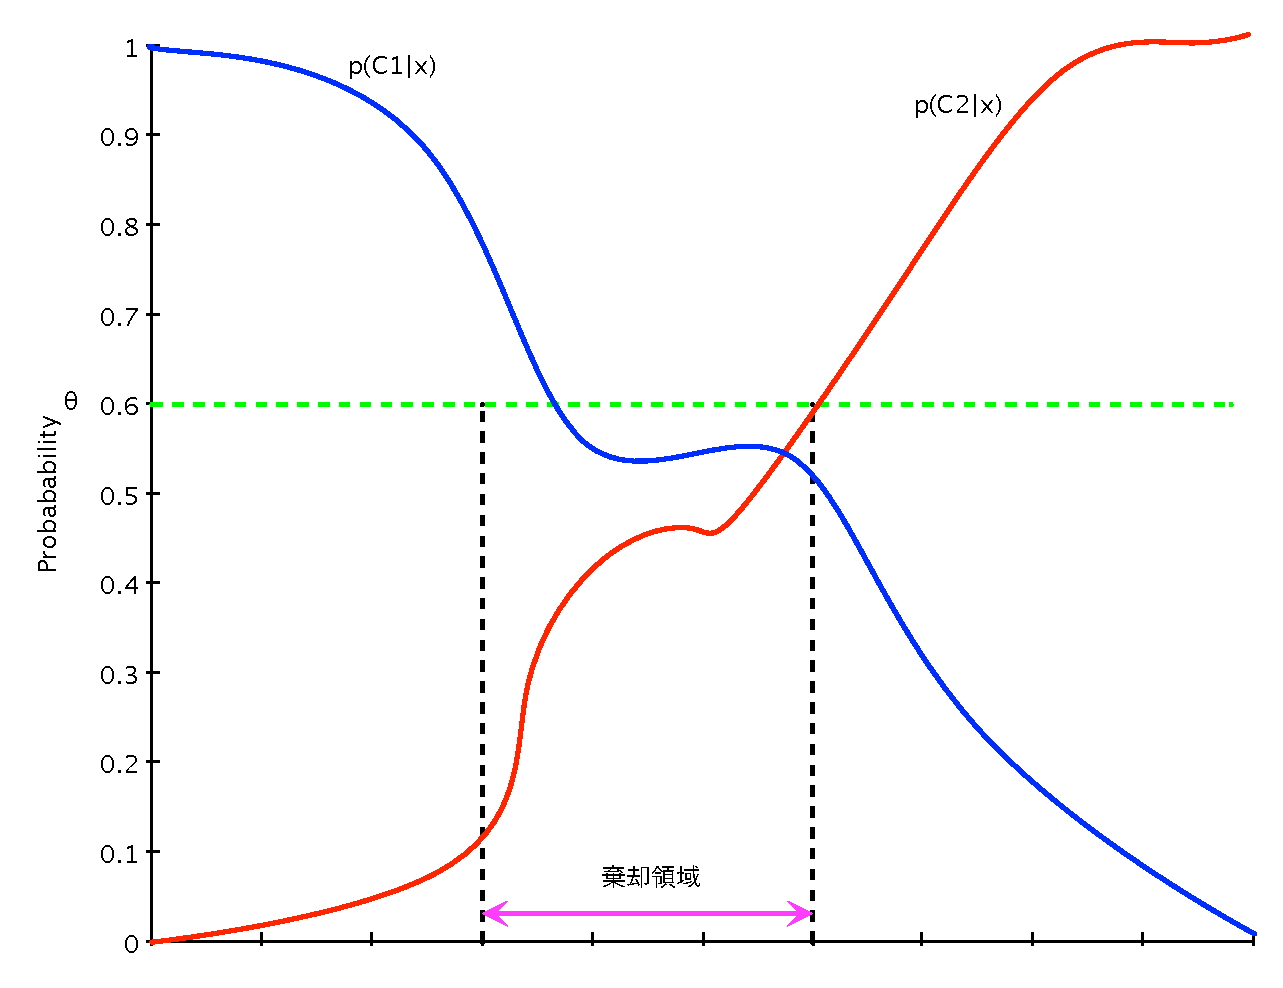
\includegraphics[width=4.5cm,clip]{res/reject_option.eps}
  \end{figure}
  \end{description}
\end{frame}

\begin{frame}
  \frametitle{1.5.4 inferense and decision}
  推論段階$\to$決定段階への3つのアプローチ
  \begin{description}
    \item[生成モデル(generative model)] \hfill \\
       クラスごとにクラスの条件付き密度$p(x|C_k)$を決定する推論問題を解く。そして$p(C_k)$も求めて、事後確率$p(C_k|x)$を求める。そして決定理論によりクラスに割り当てる。出力だけでななく入力もモデル化されるので、データの生成も可能になる。
    \item[識別モデル(discriminative model)] \hfill \\
      クラス事後確率$p(C_k|\bm{x})$を決定する推論問題を解き、決定理論を用いて新たな$\bm{x}$をクラスに割り当てる。
    \item[識別関数(discriminative function)]
      推論せずに直接決定する。各入力$\bm{x}$から直接クラスラベルへと写像する。
  \end{description}
\end{frame}

\subsection{1.6 情報理論}
\begin{frame}
  \frametitle{情報量とエントロピー}
  ある離散確率変数$x$があるとする。

  $h(x) = -\log_{2}p(x)$ : 情報量を表す
  
  $H[x] = - \sum_{x} p(x)\log_{2}p(x)$ : 確率変数$x$のエントロピー
\end{frame}

\begin{frame}
  \frametitle{}
  確率変数$x$を与え、8個の可能な状態を等確率で取る。
  
  その値を受信者に3bitの長さにして送る。\\この変数のエントロピーは、
  \begin{gather*}
    H[x] = -8 \times \frac{1}{8}\log_{2}\frac{1}{8}=3bit
  \end{gather*}

  次に$x$は${a,b,c,d,e,f,g}$の8この可能な状態をとり、$\{\frac{1}{2},\frac{1}{4},\frac{1}{8},\frac{1}{16},\frac{1}{64},\frac{1}{64},\frac{1}{64},\frac{1}{64} \}$の確率で与えられる。
  その際のエントロピーは
  \begin{align*}
    H[x] &= -\frac{1}{2} \log_{2} \frac{1}{2} -\frac{1}{4}\log_{2}\frac{1}{4} -\frac{1}{8}\log_{2}\frac{1}{8} -\frac{1}{16}\log_{2}\frac{1}{16} -\frac{4}{64}\log_{2}\frac{1}{64} \\
         &= 2bit
  \end{align*}
  確率の分布が非一様なものよりも、一様な分布のほうがエントロピーは高い事がわかる。
\end{frame}

\begin{frame}
  \frametitle{}
\end{frame}

\begin{frame}
  \frametitle{}
\end{frame}

\begin{frame}
  \frametitle{}
\end{frame}

\begin{frame}
  \frametitle{}
\end{frame}

\begin{frame}
  \frametitle{}
\end{frame}

\begin{frame}
  \frametitle{}
\end{frame}

\begin{frame}
  \frametitle{}
\end{frame}

\begin{frame}
  \frametitle{}
\end{frame}


\end{document}
